\documentstyle[epic,eepic,graphicx,cite,amsmath,caption,subcaption,algorithm,algorithmicx,algpseudocode,longtable,appendix,url,listings]{report}
%\mathindent 0pt
\input{epsf}


\renewcommand{\baselinestretch}{1.6}
\newtheorem{theorem}{Theorem}[chapter]
\newcommand{\btheorem}{\begin{theorem}\rm}
\newcommand{\etheorem}{$\diamond$\end{theorem}}
\newtheorem{definition}{Definition}[chapter]
\newcommand{\bdefn}{\begin{definition}\rm}
\newcommand{\edefn}{\end{definition}}
\newtheorem{lemma}{Lemma}[chapter]
\newtheorem{remark}{Remark}[chapter]
\newcommand{\bremark}{\begin{remark}\rm}
\newcommand{\eremark}{\end{remark}}
\newtheorem{example}{Example}[chapter]
\newcommand{\bexample}{\begin{example}\rm}
\newcommand{\eexample}{\end{example}}
\newtheorem{assumption}{Assumption}[chapter]
\newcommand{\bassump}{\begin{assumption}\rm}
\newcommand{\eassump}{\end{assumption}}
\newcommand{\ekf}{Extended Kalman Filter }
\newcommand{\slam}{Simultaneous Localization and Mapping }
\newcommand{\imp}{Integrated Mobile Platform }
\graphicspath{{./Images/hardware/}, {./Images/imageprocessing/}, {./Images/IMP/},{./Images/kinematics/},{./Images/modeling/},
{./Images/pathplanning/},{./Images/results/}}
%\newtagform{defaultoveride}{}{}
%\usetagform{defaultoveride}
\begin{document}
\title{Path Planning and Object Detection for a Robotic Manipulator}
\author{Alaina Herkelman}
\maketitle
%\mstitlepage
\topmargin=0.4 in
\textwidth=6.0 in
\textheight=9.0 in


\setcounter{page}{1}
\pagenumbering{roman}
\include{./Roman/publications}
\include{./Roman/acknowledgements} 
\begin{abstract}

Path planning is a crucial part of controlling a robotic manipulator. To move in an unknown environment sensors must be utilized for generating workspace information. In this report an A start based path planning algorithm was implemented for a four degree of freedom manipulator. A three dimensional camera was used to locate the goal and obstacles within the manipulators workspace. The results of real world implementation, modeling and the theory behind them are discussed.
\end{abstract}
\tableofcontents
\listoffigures
\listoftables
\newpage
\setcounter{page}{1}
\pagenumbering{arabic}
\chapter{Introduction}
 Robotics is becoming a more popular and useful field in the world today. Sensors have become more accurate and practical for mapping environments allowing robots to be used in more situations. Robotic manipulator's are used for situations where repetitive or dangerous tasks can be replaced with robotic . This is most commonly found in areas such as manufacturing. Combining manipulators with machine vision allows manipulators to adapt to different environments by visualizing the workspace.
 
 For this project a four degree of freedom robotic manipulator was used to grab objects within its workspace while avoiding other found obstacles. A three dimensional camera was used to gather data about the manipulator's workspace. Computer vision algorithms were developed to locate known objects within the camera's field of view. A path planning algorithm was then set up to calculate a path from the current arm position to a goal object and pick it up. 
 
 The algorithm used for path planning was a graph search method with an addition of a potential fields component to help the arm avoid obstacles while still moving towards the goal. The vision algorithms located goal objects and obstacles by using color and basic shape detection.  
 
 The report follows the following setup: Chapter 2 discusses different methods of path planning and object detection in images, Chapter 3 shows the results of the kinematic models of the manipulator, Chapter 4 goes over the hardware setup for this project, Chapter 5 states the results of developing image processing algorithms, Chapter 6 overviews another application for computer vision in robotics, Chapter 7 goes over the development of the path planning algorithm, Chapters 8 and 9 discuss the results of the path planing in simulation and real world implementation, Chapter 10 is the conclusion of the project.
\chapter{Literature Survey}

Path planning is a way to generate a path for a robot to meet certain input conditions. It is often desired to move the robot from one place to another while going around any objects that may be in the way. The steps to do this can be broken into two major components: finding information about the workspace and using an algorithm to develop the path. 

Path planning can be done in both static and dynamic environments. A static environment is one that does not change. Once the workspace has been visualized it is assumed none of the objects move. In a dynamic environment the surroundings of the robot do change. This means that the workspace information will change in position as the robot moves. It then becomes necessary to both visualize and plan a path simultaneously, requiring better speed and flexibility for both the path planner and vision methods.

\section{Visualizing a Workspace}
Generating data about a workspace requires some type of sensor, or sensors, which can provide data about the robot's surroundings. The most common methods for this involve vision sensors and distance sensors. The overall goal is to create some knowledge of the 3 dimensional workspace of the robot. Camera's are useful in locating obstacles but need some method to convert from pixels to real world coordinates. To locate a goal in an environment using computer vision requires some method of object recognition. There are a number of different methods and programming libraries to help with this problem. A few common methods are described below.

\subsection{Color Based}  
One method of finding on object in an image is based on color. The range of pixel values for a certain color can be saved to an algorithm that searched through an image to find pixel values within that color range. To create accurate data from this requires some amount of filtering and correction on the image to reduce the impact noise. The major downfall of this method is that the color must be known to find the object and if any objects, besides the desired, are in the same color range the results of the detection will not return the right data. This method is therefore most useful in controlled environments where the colors of objects in the image can be selected.

\subsection{Geometery Based}
An alternative to finding by color is finding by shape. The basic principle of this is to search through the edges of an image for geometric shapes. This can be done to find any primitive shapes in an image. A more complex shape can be broken into a combination of geometric primitives to be located using this method. To find a primitive shape in an image a method for edge detecting must be used. From found edges in the image these can be searched to find the contours matching the desired simple shape.

\subsection{Feature Based}
This method finds a known object in an image by comparing known 'features' of the object to an image. An algorithm is run to find distinctive parts of an object from a picture of it. These features are commonly lines, points, shapes but can be anything else generated. An array of these features can be saved and compared to features in another image. If enough of the object's features are found then the object is said to be found in the image. This method is a bit more complicated but works best for finding complex objects in a more cluttered environment.      

\section{Path Planning}
There are many different solutions that have been developed to solve the path planning problem. Two of the most popular are potential fields and graph search. These methods can be broken down into more specific algorithms but all share similar aspects.

\subsection{Potential Fields}
The potential fields method uses an equation to calculate the next step of the path by repelling the solution away from obstacles while attracting it to the goal. The equation acts as a cost function of which the global minimum is the goal. The cost will increase the closer the obstacles and the cost will decrease the closer to the goal. The cost functions is comprised of two parts; an attractive field and a repulsive field. 

The shape of equation that directly solves the attractive field is a conical, which is a concave shape with the center at the goal. The problem with this equation is that it is not continuous which causes most optimization methods to be impossible. To fix this a quadratic equation, which increases the farther from the goal, is added to the conic equation. The resulting equation for the attractive field is shown in equation \ref{eq:attract}.
\begin{equation}
\label{eq:attract}
 U_{attract}(q)  =
  \begin{cases} 
      \hfill \frac{1}{2}\zeta dist(q,q_0)^2    \hfill & if dist(q,q_0)\leq d* \\
      \hfill d*\zeta dist(q,q_0) -\frac{1}{2}\zeta d^2 \hfill &  if dist(q,q_0) > d* \\
  \end{cases}
\end{equation}

Where $\zeta$ is a scaling factor, dist(x,y) is the distance between x and y, q is current position, $q_0$ is goal position, and d* is the distance between the conical and parabolic well.

The repulsive field is set to increase quadratically based on how close the robot is to each obstacle. For a manipulator the end effector cannot be the only chosen point looked at in terms of collision. While the goal would only need to look at the end effector for the attractive field, since that is the only part of the arm desired to be at that goal. For the obstacles no point on the link is desired to touch the obstacle. This means the whole arm, not just the end effector must be checked for collision with the obstacle. A way to do this is by calculating which point on the manipulator is closest to the obstacle and use that distance to calculate the repulsive field. The result of this is shown in equation \ref{eq:repel}.

\begin{equation}
\label{eq:repel}
 U_{repel}(q)  =
  \begin{cases} 
      \hfill \frac{1}{2}\zeta (\frac{1}{P(q)} - \frac{1}{P_0})^2    \hfill & if P(q) \leq P_0 \\
      \hfill 0 &  if P(q) > P_0 \\
  \end{cases}
\end{equation}
Where $\zeta$ is a tuning parameter, P{q} is the distance from the closest point on the robot to the obstacle, and $P_0$ is the distance at which the obstacle should no longer effect the cost.

To calculate the overall cost function the attractive and repulsive fields are added resulting in the overall cost function. This becomes an optimization problem and can be solved using optimization methods. The most widely used of these for the path planning problem is the gradient descent algorithm. 

The biggest problem with using potential fields is the local minimum problem. As gradient decent, or another algorithm for solving the path based on a potential fields problem, travels through it can get stuck in a local minimum, where no points around it are cheaper than its current yet it is not at the goal. There are a number of methods to fix this problem, such as moving away in a randomized direction and then continuing with the algorithm. 


\subsection{Graph Search}
The graph search method of path planning works by finding a minimal path between a start and end position given a set of nodes. Each of these nodes represents a different state of the object the path planning is done for. For example the manipulator in this project a node is a set of angles at a given orientation of the arm. The connection cost between each of these nodes must also be known, often calculated by distance. Nodes can either be calculated as the search algorithm is running or generated before searching. The latter becomes impractical for problems with a high number states and typically nodes are calculated while searching. There are many different algorithms based on this method some of which are described below.

\section{Dijkstra's Algorithm}
Dijkstra's algorithm is a search method which is guaranteed to find the optional path. To do this it starts at the start node then looks at all of the neighbors. It saves all of the neighbors of the start node and records the cost to get there. It then looks at the least cost of the saved nodes, removes it from the saved set, and saves all of its neighbors. This is repeated until the goal is selected as the point with the least cost.. If at any point a node is found to have a cheaper cost when reached through a different set of neighbors the new lower cost is saved as the cost to node. When the goal is found the cost to all nodes from the start to end have their costs known. The optimal path can then be constructed by moving backwards from the found end node. While this is guaranteed to find the least cost path between start and end this algorithm also looks at a large amount of unnecessary nodes as it looks at neighbors in all directions. This algorithm is accurate but inefficient. 

\section{Greedy Algorithm}
On the opposite end of the speed versus accuracy spectrum is the Greedy Algorithm. It works by beginning at the start node and looking at the neighboring nodes. It then moves to the neighbor with the least cost and throws out all of the others. It keeps doing this until the end node is reached. This method creates the optimal path in the optimal amount of time given a very direct path is the optimal solution.  As this is often not the case the greedy algorithm is not a practical search algorithm.

\section{A*}
The A* method follows the same steps as Dijkstra's algorithm where is saves all of the neighbors of the node it is currently looking at. Unlike in Dijkstra's algorithm the cost is calculated a function of both the cost to reach the node and an estimate of the cost to the distance. This means the cost is more for nodes going away from the goal and less for the nodes towards the goal. This significantly reduces the number of nodes that are looked at as when tuned properly only likely nodes will be looked at. The A* algorithm provides a balance between accuracy and time as it only looks at nodes it views as potential candidates for reaching the goal quickly. If tuned correctly A* will return the optimal path. 
\chapter{Kinematics}
The manipulator used was a four degree of freedom (DOF) arm with a gripper attached as the end effector. All joints were revolute and implemented by servo motors. A drawing of the arm is shown in Figure \ref{fig:ARM}. To properly control the manipulator the forward and inverse kinematics were derived.

\begin{figure} [h]
\centering
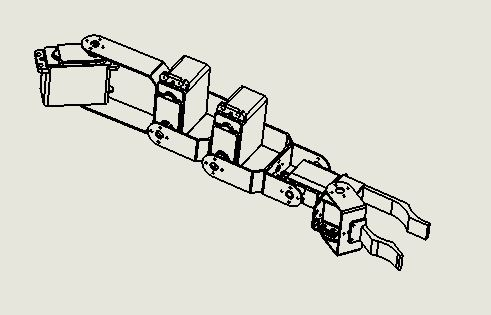
\includegraphics[width=0.5\textwidth]{armdrawing}
\caption{The Mobile Manipulator}
\label{fig:ARM}
\end{figure}

\section{Forward Kinematics}
Forward kinematics is finding the position and orientation of a manipulator's end effector given the position of all of its joints. For this manipulator the end effector position was calculated in terms of the angles of the first four joints of the manipulator $\theta_1$ - $\theta_4$. The gripper was considered only as a length as it has no effect on the arm's overall position or orientation. An manipulator simplified as a drawing of its joints can be seen in Figure \ref{fig:ARMCoord}.

\begin{figure}
\centering
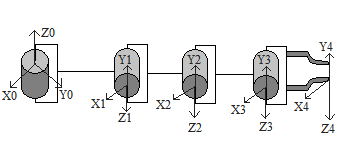
\includegraphics[width=0.5\textwidth]{manipulatoraxis}
\caption{The Mobile Manipulator with Coordinate Frames}
\label{fig:ARMCoord}
\end{figure}

The coordinate frames of each of the joints were found using the Devavit-Hartenberg (D-H) convention. The resulting coordinate frames and DH parameters are also drawn in Figure \ref{fig:ARMCoord}. The D-H table, which contains each of the D-H parameters for calculating the transformation matrix of each joint is shown in Table 1. The matrix for each joint was then calculated using the formula in equation \ref{eq:Amat} where $A_i$ is the transformation matrix between the coordinate frame $o_ix_iy_iz_i$ and $o_{i-1}x_{i-1}y_{i-1}z_{i-1}$ where $o_0x_0y_0z_0$ is the origin coordinate frame. The transformation matrix $T_4^0$, to convert from the coordinate frame of the end effector to the coordinate frame of the origin is found by multiplying all of the A matrices together. So $T_4^0$ = $A_1*A_2*A_3*A_4$. The fourth column of this matrix represents the the 3-Dimensional (3D) coordinates of the manipulator's end effector with respect to the origin coordinate frame. $R_{14}$ is the x position $R_{24}$ is the y position and $R_{34}$ is the z position where R = $\begin{bmatrix}
  r_{11} & r_{12} & r_{13} & r_{14} \\
  r_{21} & r_{22} & r_{23} & r_{24}\\
  r_{31} & r_{32} & r_{33} & r_{34} \\
  r_{41} & r_{42} & r_{43} & r_{44}
 \end{bmatrix}$. This column then returns the equations for x, y, and z in terms of the angles $\theta_1$ - $\theta_4$. As these equations are very long the matrices above were calculated for each value and multiplied in code rather than writing out the equations.
\begin{table}
\centering
\begin{tabular}{| l | l | l | l | l |}
 		\hline
 		Joint & $d_i$ & $\alpha_i$ & $a_i$ & $\theta_i$ \\ \hline
 		1 & 0 & $-90^o$ & $l_1$ & $\theta_1*$\\ \hline
 		2 & 0 & $0^o$ & $l_2$ & $\theta_2*$\\ \hline
 		3 & 0 & $0^o$ & $l_3$ & $\theta_3*$\\ \hline
 		4 & 0 & $0^o$ & $l_4$ & $\theta_4*$\\ \hline
	\end{tabular}
	\label{table:DH}
	\caption{D-H table}
\end{table}

\begin{equation}
\label{eq:Amat}
\begin{bmatrix}
  cos\theta_i & -sin\theta_icos\alpha_i & sin\theta_isin\alpha_i & \alpha_icos\theta_i \\
  sin\theta_i & cos\theta_icos\alpha_i & -cos\theta_isin\alpha_i & \alpha_isin\theta_i\\
  0 & sin\alpha_i & cos\alpha_i & d_i \\
  0 & 0 & 0 & 1
 \end{bmatrix}
\end{equation}

\section{Inverse Kinematics}
The inverse kinematics of a manipulator are a way to calculated the position of each of the joints of a manipulator in terms of end effector position. The inverse kinematics of this manipulator were simple enough to be calculated analytically. The process of this is discussed below.

The last three angles of the manipulator $\theta_2$, $\theta_3$, and $\theta_4$ all lie within the same plane as each other. This plane's location in 3D space is determined by $\theta_1$ which only moves in the x-y plane. The projection of the arm onto the x-y plane is shown in Figure \ref{fig:xy} where $x_c$ and $y_c$ are the desired x and y coordinates of the end effector. From this drawing it is easy to see that $\theta_1$ can be calculated as the inverse tangent of $\frac{(x_c)}{y_c}$ or $\theta_1 = Atan2(x_c,y_c)$ where Atan2 is the inverse tangent function taking signs into consideration.

The remaining three angles can be projected into the plane formed by the z-axis and the plane determined by $\theta_1$ in the x-y axis. This is seen in Figure \ref{fig:z} where r = $\sqrt{x^2+y^2} - l_1$ which is the length of the projected manipulator on the x-y plane. Two equations can be found for $z_c$ and r using geometric properties on the projected image. Since only two equations can be found and there are three unknown variables the desired orientation of the end effector $\theta_c$ must be specified. The resulting three equations are shown in equation \ref{eq:Zproj}.

\begin{subequations}
\label{eq:Zproj}
	\begin{align}
	z_c = l_2sin\theta_2+l_3sin(\theta_2+\theta_3) + l_4sin\theta_c\qquad \\
	r = l_2cos\theta_2+l_3cos(\theta_2+\theta_3) + l_4cos\theta_c\qquad \\
	\theta_c = \theta_2 + \theta_3 + \theta_4 \qquad 
	\end{align}
\end{subequations}

\begin{figure}
    \centering
    \begin{subfigure}[b]{0.3\textwidth}
    	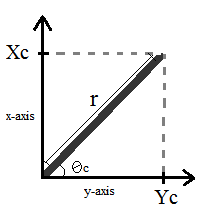
\includegraphics[width=\textwidth]{xyaxis}
    	\caption{Projection of Manipulator onto the XY axis}
   	 	\label{fig:xy}
   	 \end{subfigure}
   	 \quad
    \begin{subfigure}[b]{0.3\textwidth}
		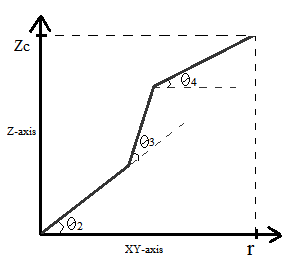
\includegraphics[width=\textwidth]{zprojection}
		\caption{Projection of Manipulator onto the Z-plane Axis. }
		\label{fig:z}
    \end{subfigure}
    \quad %add desired spacing between images, e. g. ~, \quad, \qquad, \hfill etc.
      %(or a blank line to force the subfigure onto a new line)
 	\caption{Projections for solving the inverse kinematics geometrically.}
\end{figure}
These equations were solved for $\theta_2$, $\theta_3$, and $\theta_4$.  The final results for the inverse kinematics; $\theta_1$, $\theta_2$, $\theta_3$, and $\theta_4$ in terms of $x_c$, $y_c$, $z_c$, and$\theta_c$ are shown in equation \ref{eq:inverse}.

\begin{subequations}
\label{eq:inverse}
	\begin{align}
	\theta_1 = Atan2(y_c,x_c)\qquad \\
	\theta_3 = cos^{-1}(\frac{(z_c-l_4sin\theta_c)^2+(r-l_4cos\theta_c)^2-l_2^2-l_3^2}{2l_2l_3})\qquad \\
	\theta_2 = tan^{-1}(frac{z_c-l_4sin\theta_c}{r-l_4cos\theta_c}) - tan^{-1}(frac{[l_3sin\theta_3],[l_2l_3cos\theta_3]}) \qquad \\
	\theta_4 = \theta_c - \theta_2 - \theta_3 \qquad
	r = \sqrt{x_c^2+y_c^2}-l_1
	\end{align}
\end{subequations}


It also becomes helpful to have a way to calculate if the increase kinematics is possible. If the calculation of $\theta_3$ is an imaginary number than there is no real solution to the inverse kinematics. Inverse cos returns an imaginary number when taking the inverse of a number greater than one. Therefore if the denominator is bigger than the numerator than the resulting $\theta_3$ will be imaginary. So if $(z_c-l_4sin(\theta_c))^2 + (r-l_4cos(\theta_c))^2 - l_2^2 - l_3^2) < 2l_2l_3$ than the desired x,y,z coordinates are outside of the workspace of the manipulator. 

The physical constraints of the manipulator must also be taken into account. Due to the way the arm is constructed the each joints has a limit of the angles it can be set to. The are as follows; $-90^o \leq \theta_1 \leq 90^o$, $-50^o \leq \theta_2 \leq 120^o$, $-55^o \leq \theta_3 \leq 120^o$, $-110^o \leq \theta_4 \leq 90^o$. These constraints were found by finding the angle at which the joints cannot turn farther without colliding with another part of the arm. A sample of the manipulator workspace taken at all possible angles with an increment of $5^o$ is shown in Figure \ref{fig:work}.  The code for handling the kinematics of the manipulator can be seen in Appendix B.5.

\begin{figure}
\centering
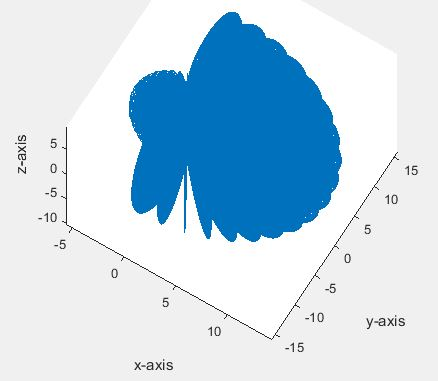
\includegraphics[width=0.5\textwidth]{workspace}
\caption{Workspace of the manipulator }
\label{fig:work}
\end{figure}
\chapter{Hardware}
The setup of the manipulator was a 3D camera mounted above the manipulator to view its workspace. A micro-controller and computer were the main methods of control. The manipulator control system is set up as seen in the diagram in Figure \ref{fig:maindiagram}. Camera data is read in and processed by the computer, the results are sent to the micro controller, which sends PWM signals to the servo motors through a power and control circuit. A diagram of connections within this system can be seen in Figure \ref{fig:diagram} The code to handle the communication of the system can be found in Appendix B.

\begin{figure}[h]
\centering
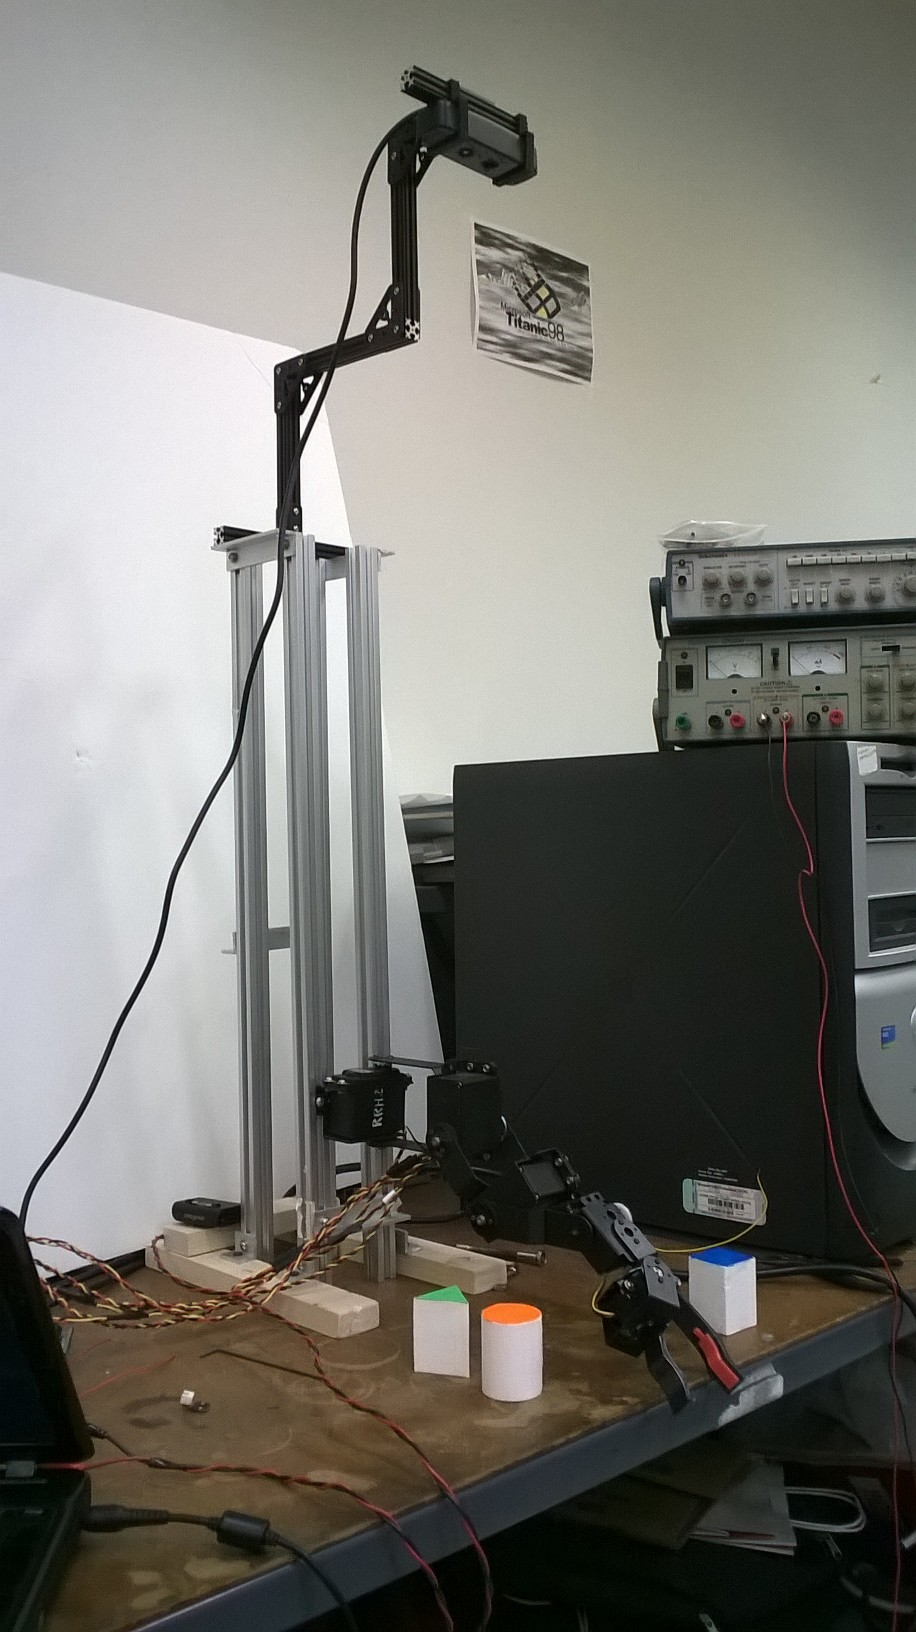
\includegraphics[height=0.5\textwidth]{actual}
\caption{The manipulator.}
\label{fig:real}
\end{figure}

\begin{figure}[h*]
\centering
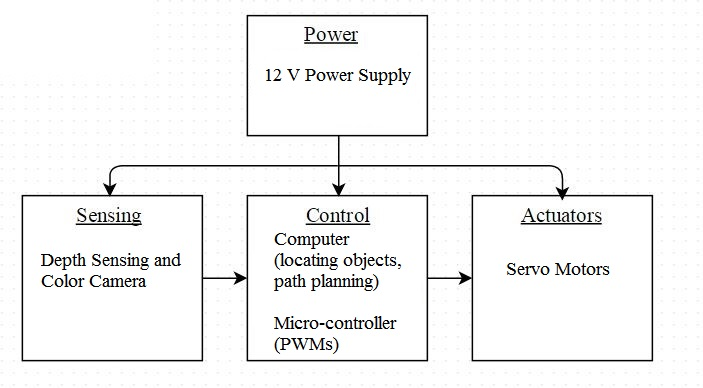
\includegraphics[width=0.7\textwidth]{maindiag}
\caption{System diagram of the manipulator.}
\label{fig:maindiagram}
\end{figure}

The servos used to construct this arm had no method of feedback. The connections of each servo were power, ground, and input signal. Unlike some more expensive servos which have a connection for some or multiple types of feedback these servos are operated as a feed forward system. This means that commands that are given are not adjusted by any kind of error provided by a feedback system. The code on the micro controller for controlling these servos can be seen in Appendix C.


\begin{figure}
\centering
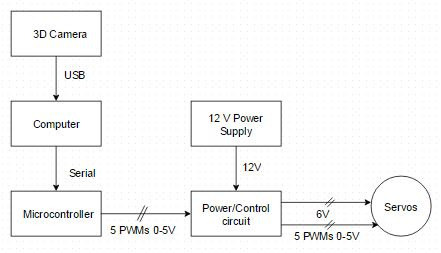
\includegraphics[width=0.6\textwidth]{diagram}
\caption{Diagram of manipulator control system.}
\label{fig:diagram}
\end{figure}

The camera used was a Creative Senz 3D depth sensing and color camera. The computer code was run on Linux using bot C++ and Python. The micro controller used was a small lab built autopilot. The processor on the autopilot was a TM4C controller. The TM4C was used to control the servos. This code was originally designed on an RM48 processor but switched over to make future integration with a mobile platform robot easier. The manipulator itself is constructed from Hitec servos and the associated brackets. A list of all components can be found in Table \ref{tab: Components}.

\begin{longtable}{| p{3cm} | p{10cm} |}
		\caption{List of major components on the robotic manipulator system.}
		\label{tab: Components}\\

 		\hline
 		 Component & Description \\ \hline 
 		\endhead
 		

 		
 		\hline \hline
 		\endlastfoot
 		
 		Baby Autopilot(BAP) & Small single processor control unit. 
	 		\\ & $ \bullet $ 80 Mhz TM4C123GH6PZ micro-controller with 32 kB internal RAM and 256 kB internal Flash  
	 		\\  & $ \bullet $ 2 UARTs  
 			\\  & $ \bullet $ 8 PWM outputs	
 		\\ \hline
		Camera & USB Color and Depth Sensing camera
			\\  & $ \bullet $ USB 2.0 and USB 3.0 compliance
	 		\\  & $ \bullet $ Max frame rate of 30fps
	 		\\  & $ \bullet $ Depth range from 6 in to 3 ft. 
 		\\ \hline

 		Servos & Servo motors  
 			\\  & $ \bullet $ Pulse Width Control 1500usec Neutral
 			\\  & $ \bullet $ 6V operating voltage
 			 			 			 		
 		\\ \hline 
	\end{longtable}
%\end{table}

The power/control circuit is mostly a 6-volt regulator with connections between the servos and micro controller. The layout is shown in Figure \ref{fig:circuit}. An enable pin and jumper were used so that the servos only receive power when an enable signal, GPIO of 3.3v, is sent from the micro controller. The jumper can also be removed to stop powering the servos in the case power needed to be shut off quickly.

\begin{figure}[h]
    \centering
    \begin{subfigure}[b]{0.3\textwidth}
    	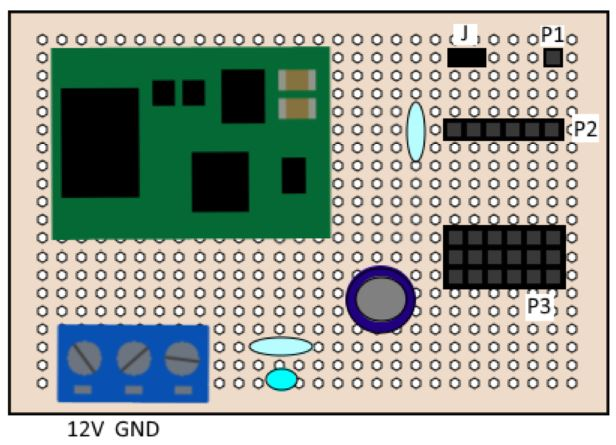
\includegraphics[width=\textwidth]{circuit}
   	 \end{subfigure}
   	 \quad

 %add desired spacing between images, e. g. ~, \quad, \qquad, \hfill etc.
      %(or a blank line to force the subfigure onto a new line)
 	\caption{Connection Circuit for Manipulator. }
 	\label{fig:circuit}
\end{figure}

The last major design component for the hardware was the manipulator's gripper. It was built from a combination of a Hitec servo, existing brackets, and 3D printed pieces. The design concept was a fixed thumb with an opening and closing finder controlled by the servo. All parts were modeled in Solidworks and the thumb and finger pieces printed. Rubber was glued onto the 3D printed pieces to increase the friction when picking up objects. The assembly of the gripper opened and closed around a cylindrical object is shown in Figure \ref{fig:gripper}. The object and similar objects were also 3D printed and used as the goal and obstacles for the arm.

\begin{figure}[h]
\centering
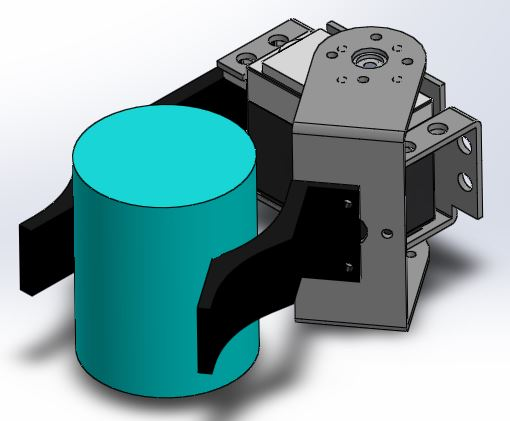
\includegraphics[width=0.4\textwidth]{gripper}
\caption{Gripper holding cylindrical object.}
\label{fig:gripper}
\end{figure}
\chapter{Image Processing}
To locate objects in the manipulator workspace computer vision methods were used. The Creative Senz 3D depth sensing camera was used to gather depth and color data of the workspace. OpenCV was then used to locate objects in the read images. The depth data could than be used to actually calculate the xyz position of the found image location. This was the general method for locating objects in the manipulator's workspace.

\section{Creative Senz 3D}
The Creative Senz 3D camera produces three different outputs which is sends using USB; sound, depth data, and color images. Each of these is read in by the computer by connecting to the corresponding data streams. To make the camera Linux compatible the DepthSense Software Development Kit (SDK) was used. This software was designed for use with SoftKinetics's 3D cameras but currently works with the Creative Senz 3D. The SDK for the Creative camera was not used as it is a Window's only program. Linux compatability was important for future work to be able to put code to interface with the camera could by run on Odroid which runs a Linux operating system. 

\section{Depthsense SDK}
The DepthSense SDK libraries provide classes and functions for handling the camera data as well as sample code for reading in the data. The main function for gathering data initializes the color and depth nodes than waits for new data of each of those to be received. The nodes for color and depth can be configured to return the desired types of data. For example the different depth data types used in this project were the UV Map, depthMap, and VerticesFloatingPoint and the color data was colorMap. The colorMap data stores the Red Green Blue (RGB) values for each pixel in the color image. The depthMap and verticiesFloatingPoint stores the xyz coordinates of each depth point as calculated in the SDK. The UVMap data is used to convert between the depth image and color image. This is necessary because the depth image is not taken at the exact same place on the camera as the color image and the two images are not the same size. Therefore to find the depth at a color pixel coordinate or the color of a point on the depth map on a way to convert between them is necessary.

The v member of the uv map refers to the row, or height, of the color image and the v refers to the column or width of the color image. The conversion algorithm between color pixel coordinates to the uv coordinate is shown in algorithm \ref{alg:uv}.

\begin{algorithm}
	\begin{enumerate}
		\item Get UV map from DepthSenseSDK.
		\item colorImageRow = V member of UV * height of color image.
		\item colorImageColumn = U member of UV * width of color image.

	\end{enumerate}
\caption{Use UV map to convert from depth location to pixel coordinates.}
\label{alg:uv}
\end{algorithm}

Reading in the color image and depth image as well as converting between locations in the two is all that is necessary from the Depthsense SDK software. This code makes up the main part of the camera code. The main function calls the functions necessary to set up the nodes and then waits for data. Functions exist called OnNewDepthSample and OnNewColorSample which run every time new data of this type is received. It is in these functions where data was read into variables to be used for further analysis.

\section{Finding Depth Data at a Desired Location}
Once an object is located in the color image the xyz coordinates must be found. To do this the depth map is searched through and using the uv mapping technique discussed above the row and column of the color image is found for each depth point. If the row and column matches the xy position of the found object than that depth position in xyz coordinates, found by using the verticiesFloatingPoint depth data, is stored as the real world position of the image coordinates.

 For more consistent readings of depth an average of the points around the found object was used rather than just the center point. This is because there are some holes in the depth data, where it reads a default 0,0,0 coordinate. This happens most often when an object starts approaching the lower limit of range on the camera. The average was a way to avoid no data being returned in these situations. The area used was $\pm$ a third of the found objects bounding circle radius. This gives enough points to create a safe average while guaranteeing the area is always within the desired object regardless of size. 
 
 \begin{algorithm}
 	\begin{enumerate}
 		\item x,y = found pixel position in color image
 		\item radius = radius of objects bounding circle
 		\item boundaries = x,y$\pm$radius/3
 		\item for all depth data
 		\item use uv map to  find corresponding pixel location
 		\item if in boundaries save VerticesFloatingPoint to averaging point
 		\item take average of found XYZ coordinates 
 		\item filter found  coordinates
 	\end{enumerate}
 \caption{Find world coordinates of a pixel coordinate}
 \label{alg:cam}
 \end{algorithm}
 
 The found xyz position was also put through a low pass filter as the coordinates had a fair amount of noise. The filter used was a 3rd order Butterworth Filter whose equation is shown in equation \ref{eq:filter}. The derivation of this formula can be seen in Appendix 2. The algorithm for the camera coordinate to world coordinate position is shown in algorithm \ref{alg:cam}.

\begin{equation}
\label{eq:filter}
y = \frac{w_c^2x-2w_c^2xp+w_c^2xpp-yp(2w_c^2-\frac{8}{T^2})-4-ypp(w_c^2-\frac{2\sqrt{2}wc}{T}+\frac{4}{T^2})}{\frac{4}{T^2}+\frac{2\sqrt{2}w_c}{T}+w_c^2} 
\end{equation}
Where x is the current value, xp is the previous value, xpp is the previous previous value, yp is the previous filtered value, and ypp is the previous previous filtered value.

The final step in getting a usable xyz position is to convert from the camera coordinate frame to the base frame of the manipulator. The camera's coordinate frame is at the center point between the depth and color camera's and the manipulators coordinate frame is at the first joint of the manipulator. These frames are shown in Figure \ref{fig:mount}. The conversion between these frames is found by the equations in  \ref{eq:conv}.

\begin{subequations}
\label{eq:conv}
	\begin{align}
	x_{arm} = y_{cam} + a \qquad \\
	y_{arm} = x_{cam}  \qquad \\
	x_{arm} = z_{cam} - b 
	\end{align}
\end{subequations}

 Where distance a is the distance between $x_{arm}$ and $y_{cam}$ measured along the $z_{arm}$ axis and the distance b is the difference between $z_{arm}$ and $z_{cam}$ measured along the $x_{arm}$ axis. 

\begin{figure}
\centering
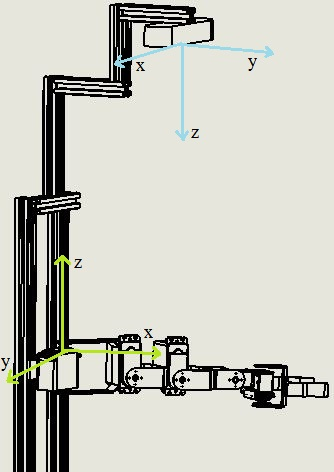
\includegraphics[width=0.3\textwidth]{armcoord}
\caption{Arm with Camera Mounted Above.}
\label{fig:mount}
\end{figure}

\subsection{Point Cloud Library}
The Point Cloud Library (PCL) is a library used for interpreting and using point clouds. Point clouds are a set of points in 3D space. These can refer to a pure depth image or also contain color information. PCL has a number of functions and examples for object recognition and tracking. It was possible to import the depth data from the camera into point cloud form and view using PCL's viewing functions. The PCL functions for object recognition did not turn out to be reliable for this project. The alternative looked at was Open Source Computer Vision (OpenCV) which more reliably found objects with the camera data. 

\subsection{Open CV}
OpenCV is another library with image processing functions which works across different computer languages and operating systems. The DepthSense SDK was written in C++ so the C++ version of OpenCV functions were utilized in this project. OpenCV has a number of different functions such as color detection, finding contours, shape fitting, and image filtering. Many of these functions were used for object detection in this project.

\subsection{First Version}
The first version of object detection was written based on color. First the color image was save as a Mat, or matrix type, which is how OpenCV saves images. The image was then converted from an RGB to HSV (Hue, Saturation, and Value). HSV has an advantage over RGB for color detection as it is easy to cover a range of saturations for a particular color, or hue, by only changing the saturation value rather than recalculating the RGB values for a slight change in saturation. The HSV range of the color was saved and compared to the pixels in the color image. A matrix of the same size was saved with a one if the pixel was in range and a zero if it was not. The result is a binary image, which is viewed as a black and white image, white for a value of one and black for a value of zero. This image was then put through filtering functions to remove holes and small objects caused by noise in the color image and the result is the object found in the image of that color.

The contours of the binary image were then found. Contours are the enclosing shapes found around the edges of an image. Assuming only one object of the desired color is in the image all found contours were merged. The OpenCV function to find the minimum enclosing circle around a contour was used to return the center point and radius of the found object. 

\begin{figure}
    \centering
    \begin{subfigure}[b]{0.3\textwidth}
    	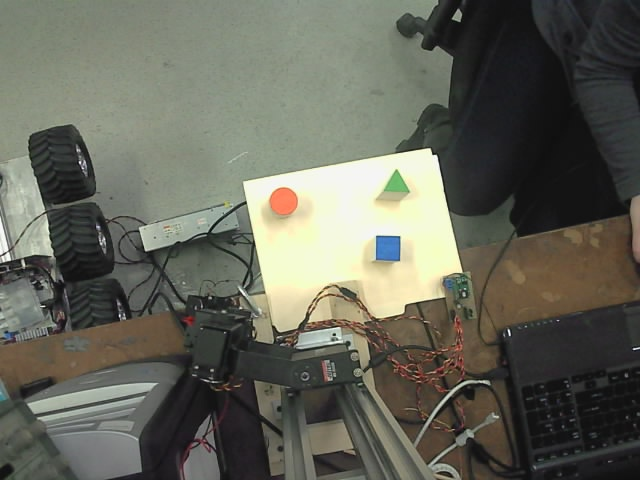
\includegraphics[width=\textwidth]{origional}
    	\caption{Original color image. }
    	\label{fig:image1}
   	 \end{subfigure}
   	 \quad
    \begin{subfigure}[b]{0.3\textwidth}
		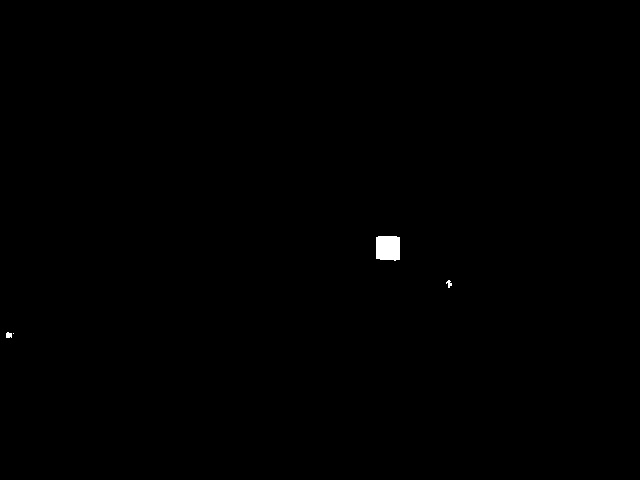
\includegraphics[width=\textwidth]{threshold}
		\caption{Binary image of found blue color before filtering. }
		\label{fig:image2}
    \end{subfigure}
    \quad %add desired spacing between images, e. g. ~, \quad, \qquad, \hfill etc.
    \begin{subfigure}[b]{0.3\textwidth}
        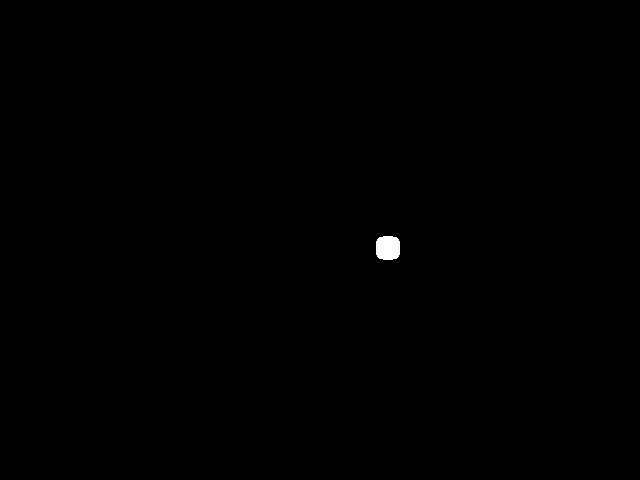
\includegraphics[width=\textwidth]{filteredthreshold}
        \caption{Binary image of found blue color after filtering.. }
        \label{fig:image3}
    \end{subfigure}
    \quad
    \begin{subfigure}[b]{0.3\textwidth}
       	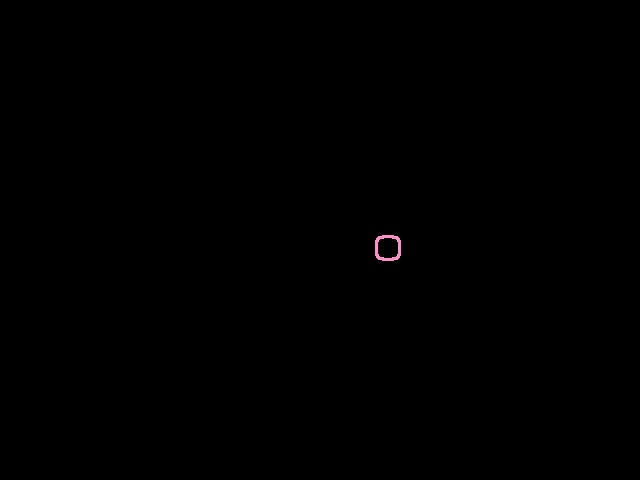
\includegraphics[width=\textwidth]{contourimage}
       	\caption{Found contours of blue object. }
       	\label{fig:image4}
   \end{subfigure}
    \quad
    \begin{subfigure}[b]{0.3\textwidth}
        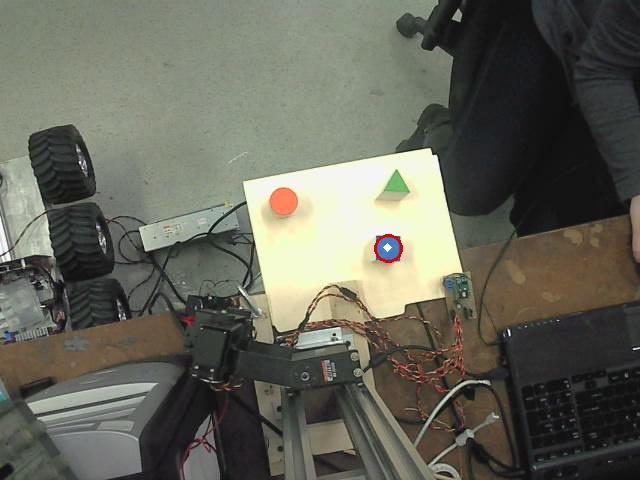
\includegraphics[width=\textwidth]{final}
        \caption{Minimum enclosing circle drawn around found object in original image. }
        \label{fig:image5}
    \end{subfigure}
    \quad
      %(or a blank line to force the subfigure onto a new line)
 	\caption{Locating a blue object in camera image. }
 	\label{fig:imag}
\end{figure}


The code for this object location program is shown in Appendix C. While this code worked consistently it did have limitations. As stated above it relies on the assumption that only one object of the desired color is present in the camera image. If there is more than one the center point returned will be somewhere in between with a radius big enough to contain all objects of that color. The program also find the minimum enclosing circle of the object regardless of its shape. This means there is no way to determine the difference between a circle, square, or any other shape in this code. It was therefore necessary to create a more well rounded algorithm for object detection.

An example of this can be seen in the images of Figure\ref{fig:imag}. To track an object of the color blue the HSV values were found to be: H = 100 - 130, S = 100-255, V = 49-255. The original image is shown in Figure \ref{fig:image1}. The thresholded image before filtering, after finding blue, is shown in Figure \ref{fig:image2} and after filtering in Figure \ref{fig:image3}. The found contours of the image are shown in Figure \ref{fig:image4} and finally the minimum enclosing circle drawn onto the image along with the found center point is shown in Figure \ref{fig:image5}. This program ran fast enough to track an object in real time and calculate 3D coordinates. Viewing the results on screen has no noticeable delay.


\subsection{Second Version}
To fix the limitations seen from the first version of the code a new version was written based on basic shape detection. The goal is to find basic shapes, such as circles, triangles, and squares from a color image. 

Shape detection started out similar to the color tracking code by creating a binary image for selected colors. For testing purposes the color selection was set to select all but the background colors. Using a binary image is much more reliable for the contour and shape detection functions in OpenCV which is why there is still a color based part to this code. This image was left unfiltered as the filtering process used in the color method rounds out the shapes too much for any kind of detection to work. Since the objects used in this project are so small in camera frame even a little bit of smoothing cuts off the corners needed for shape detection. Therefore the unfiltered image was put in the find contours function.

To then ignore all the smaller shapes only the convex contours with a larger area were looked at. Both area and convexity of a contour can be checked with OpenCV functions. For each contour meeting this criteria the approximate polygon  function was used which returns a set of vertices's for the contour. To detect the shapes the number of vertices's was used. The three shapes recognized for this program were triangle, square, and circle. The shapes were determined by the appropriate number of vertices's, for a square four and for a triangle three. The circle was marked as found for any contours with five or more vertices's. Normally this would be assumed to be a larger number but since the objects were small the approximate polygon function often found the circle to have only five vertices's. To restrict the conditions of shape further the angles between the vertices's can also be calculated. So for a square all the angles should be approximately 90 degrees, for a triangle the angles should sum to around 180 degrees, and so on. For this situation the shapes were located more easily without adding these extra conditions. There was too much noise present in the image and adding this extra angle constraint resulted in no shapes being found most of the time. Since just the vertices's condition worked much better this was the only criteria used for shape matching.

 Once found the program drew a line between all vertices's on the image and labeled it with the shape it was determined to be. An image of this working is shown in Figure \ref{fig:shapes}.

\begin{figure}
\centering
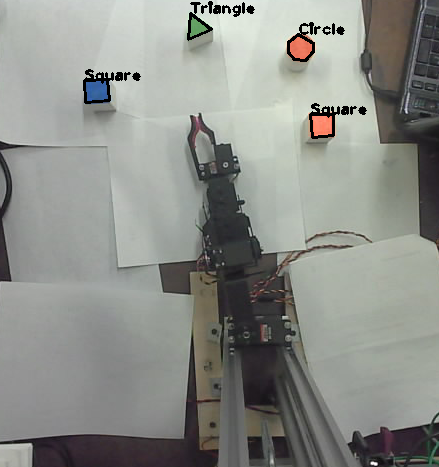
\includegraphics[width=0.5\textwidth]{shapesall.png}
\caption{Shapes located in image, labeled by program.}
\label{fig:shapes}
\end{figure}

This method often read incorrect shapes without a clean workspace. It always found the objects but did not estimate them to have the correct number of vertices. When putting the objects onto a white background enough noise was eliminated to make this method much more reliable.

To find the coordinates of the center of the shape a geometric method can be used based on the shape found. For a square the center is found as halfway from the distance of two adjacent sides. A triangle center is found as halfway between the center of one side and the opposite point. The simplest method for finding the center of the circle was to use the minimum bounding circle function on the circle contour. 

To locate all of the objects in the workspace for this experiment a combination of color and shape locating was used. Given an object for input first the color of the object is found and a binary image created for just that color. That image is then searched for the corresponding shape of the obstacle and the center point is returned. With this modification more than one object of the same color can be present in the image and an accurate result produced. 

 While this code was tested with the same workspace as used for the manipulator, the first version of the code was used for this project. The first version had less room for error and was simpler to implement. This version does provide a future more robust alternative. The code for both versions of the image code can be found in Appendix A.

\chapter{Finding Ground Truth for a Mobile Platform}
The image code written in Open CV was not just for use with object detection for the manipulator. The first Open CV code for color detection was used in a program to calculate the ground truth, or path traveled, by a mobile platform from an overhead video. The first object recognition code works for this purpose because the environment for these tests was controlled, meaning the robot was the only object of a color in the video. The ground truth is important to have so that it can be compared to results of path reconstruction based on sensors on the robot.

For this situation a red rectangle was placed on top of the platform and video taken from above the test area using a GoPro camera. Loading the video file into the open CV program after. The video was analyzed one frame at a time to locate the robot and record its center position. The colored rectangle was positioned on the robot in such a way that the center of the rectangle was also the center of the robot.
 
\section{First Solution}
Unlike with the color tracking using the depth camera the pixel coordinate of the desired location is not enough to get a estimate of the real world xyz position of the point as there is no depth data. It was therefore necessary to find another way to accurately measure the world coordinates of the robots center. The first method tried for this was using a least squares method to derive a linear equation to convert between pixel and world coordinates. The world coordinates were only calculated as an xy point as the robot traveled across a smooth surface and the z value was constant. A set of about 20 points were taken from the image at points where the world coordinates were known. Since the floor of the test area had tiles of a known size so the corners were used as the known points. 

The conversion was setup as y = Ax+B where y is the vector of real world xy coordinates, x is the pixel uv values, and A and B were matrices found using least squares. The matrix $\tilde{A}$ which equals $[A|B]$ was solved by $YX(XX^T)^{-1}$ where $XX^T$ is an invertible matrix and Y and X are full of known conversion points. These calculations were done to find A and B in Matlab and then put into the path finding code to convert to world coordinates.

This method had a number of problems; mainly inaccuracy and manual work. The linear system calculated did not provide a good estimate for converting to world coordinates. At times the result was eight inches from the actual xy coordinate. The desired accuracy range was to be with two inches of the actual value. Each time a new data was acquired the A and B matrices had to be recalculated. This is because the camera's position changes enough each time it was mounted above the test area to make the old matrices unusable. This meant that for each new run points would need to be found by hand to resolve for the A B matrices before being able to run the tracking program.

\section{Second Solution}

To address these issues the first step was to mount the GoPro in such a way that its positioning in the test area was always the same, or at very least close enough to the same to produce a manageable error. The mount that comes with the GoPro has multiple bendable joints so even if mounted at the same location the camera is not likely to be in the same orientation. A more stationary mount for the GoPro was designed in Solidworks. The design was to have a case to hold the GoPro which was attached to a clip that fit around the overhead light in the test area. The point at which the clip attached to the light was marked on the light and allowed the camera to be mounted at the same height and angle for all test runs in the environment. Figure \ref{fig:mount} shows the Solidworks model for this mount which was then 3D printed and used to hold the camera.

\begin{figure}[h]
\centering
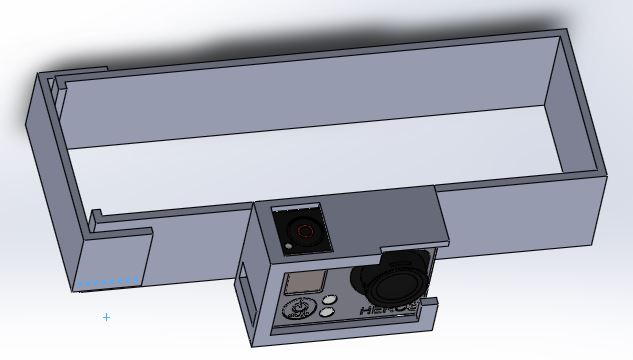
\includegraphics[width=0.5\textwidth]{camera}
\caption{Solidworks model of GoPro mount.}
\label{fig:mount}
\end{figure}

With the camera in a fixed location a more accurate way to convert the pixel coordinates to world coordinates was developed. To account for the changes in position caused by the height of the mobile platform about thirty-five data points were gathered to convert the center of an objects pixel coordinates to the real world coordinates. The object used for this was the same height was the robot to create the same offset. This offset can be seen in Figure \ref{fig:offset}. The bottle was placed at the corner of four tiles yet since the camera is not directly above it the object's center does not appear to be at the corner. The first version of the code did not account for this distortion and added to its inaccuracy. 

\begin{figure}[h]
    \centering
    \begin{subfigure}[b]{0.45\textwidth}
    	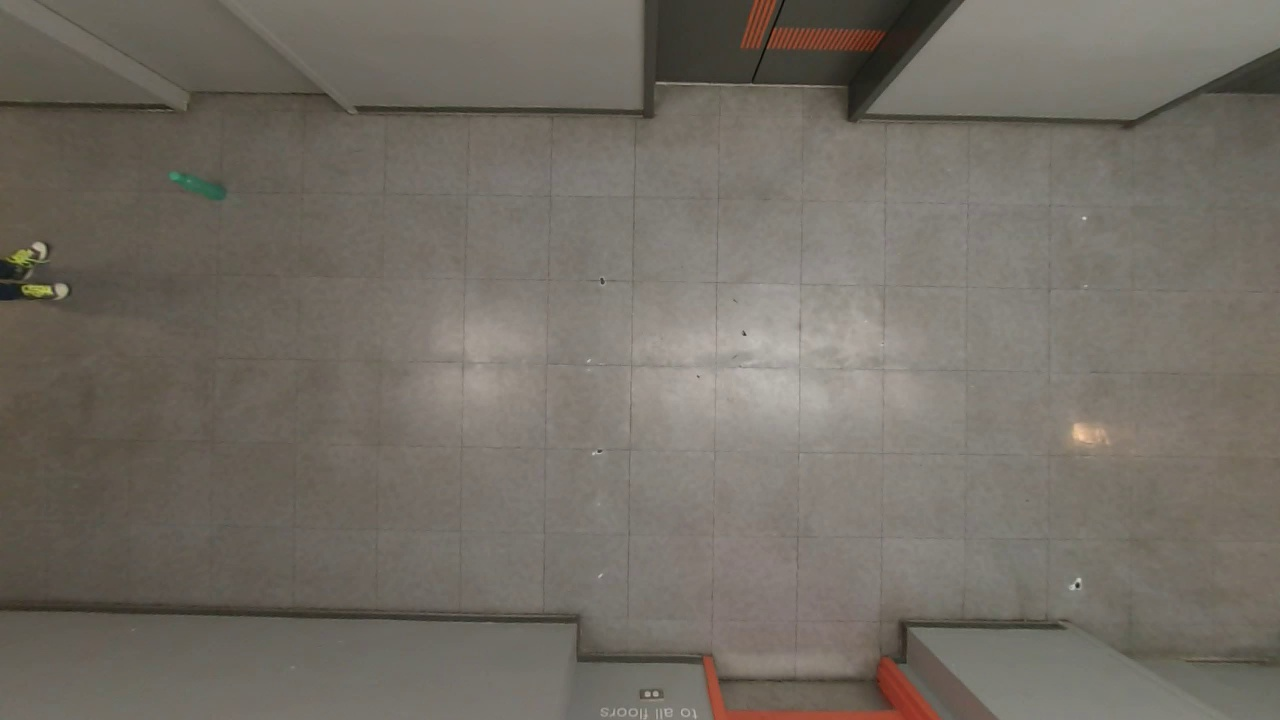
\includegraphics[width=\textwidth]{testArea}
    	\caption{Demonstration of 3D object offset. }
    	\label{fig:offset}
   	 \end{subfigure}
   	 \quad
    \begin{subfigure}[b]{0.45\textwidth}
		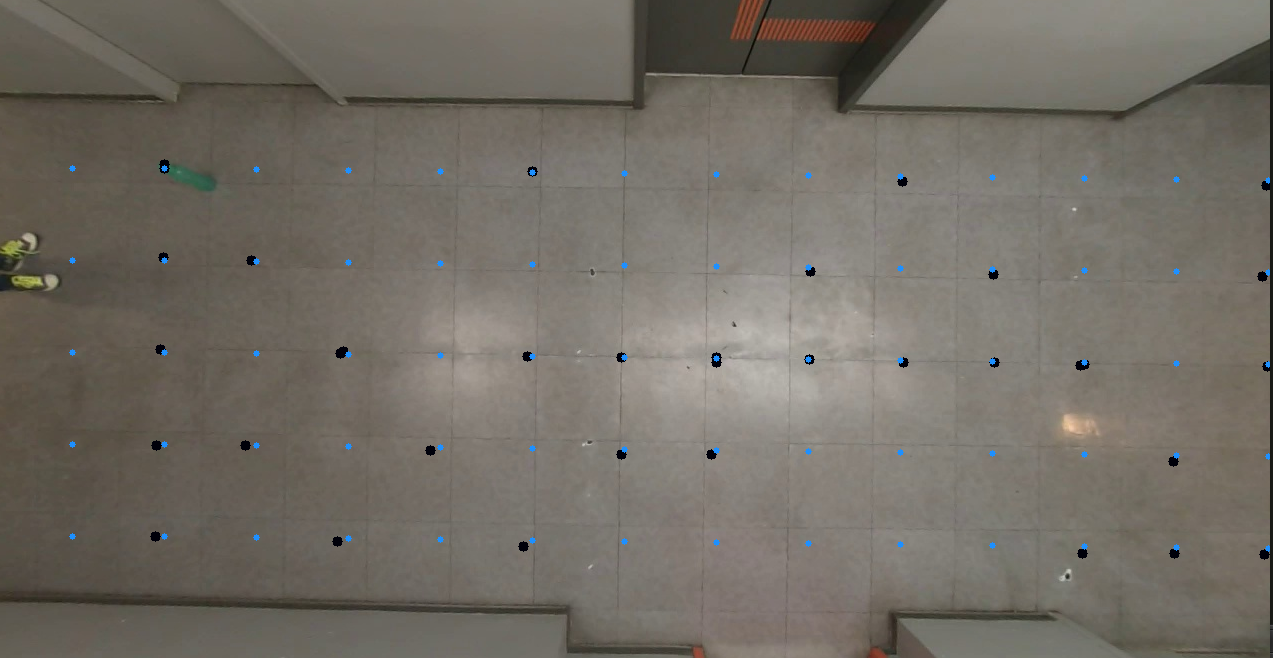
\includegraphics[width=\textwidth]{newcodepoints}
		\caption{Generated points versus manually found points. }
		\label{fig:genpoints}
    \end{subfigure}
    \quad %add desired spacing between images, e. g. ~, \quad, \qquad, \hfill etc.
      %(or a blank line to force the subfigure onto a new line)
 	\caption{View of test area from GoPro.}
 	\label{fig:images}
\end{figure}

An equation was made to generate the x and y world coordinates, The x-coordinate equation was linear and only dependent on the corresponding u pixel value. The y coordinate equation was a function of both the u and v pixel coordinates. This is because the lines found for the tiles were not perpendicular as the horizontal lines sloped slightly upwards making the y calculations a function of both x and y. A lookup table was generated for each tile corder in the test area based on these equations. Figure \ref{fig:genpoints} shows the generated points, in black, compared to those hand gathered, in blue. The lookup table could then be implemented in the main path locating program to convert to world coordinates. 

The results of this program were more accurate, within about 2 inches of the actual location, which was the desired accuracy. It was also no longer necessary to recalculate formulas for each new test in the environment. An example of the generated path is shown in Figure \ref{fig:path}. There is some jitters in the found path due to the color detection not creating the ideal data. Low pass filtering does improve the path making it smother, but there is still some inaccuracy. 

\begin{figure}
\centering
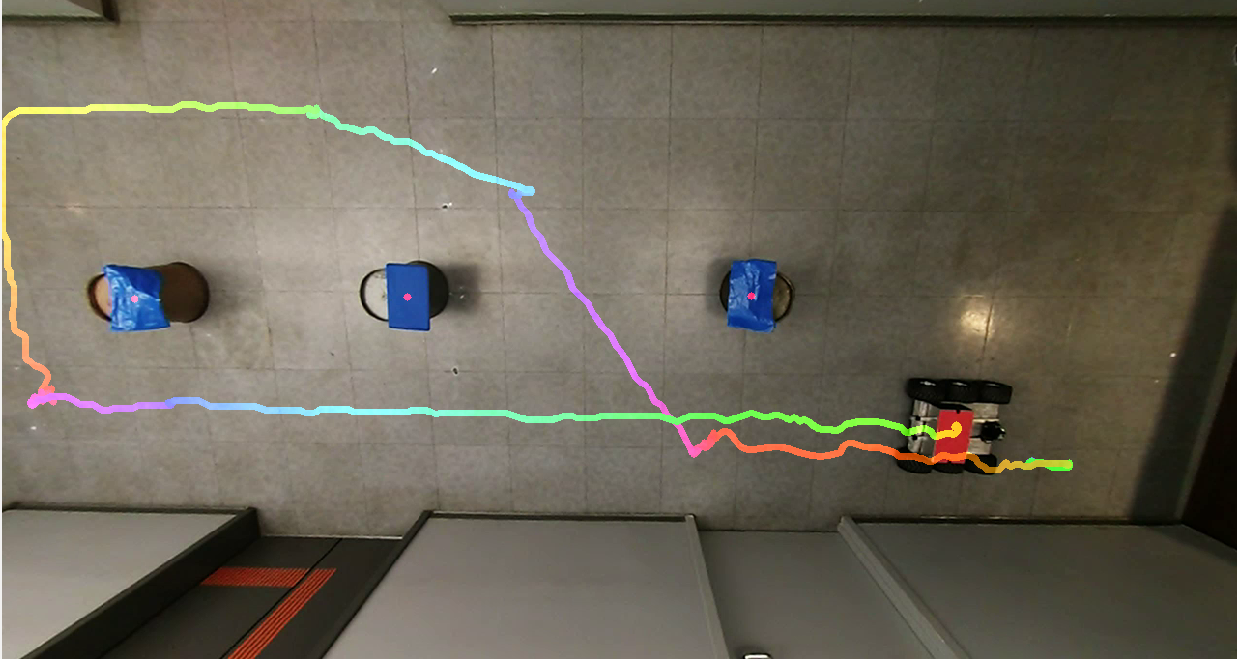
\includegraphics[width=0.5\textwidth]{path}
\caption{Found path of mobile platform drawn on camera image.}
\label{fig:path}
\end{figure}
\chapter{Path Planning}
The method selected for path planning was a graph search algorithm using A star (A*). The algorithm was first written and tested in Matlab and the rewritten to ne implemented on the real manipulator in python. 


\section{Path Planning for the Manipulator}
The first step of the path planning code was to find a way to discretize the workspace of the manipulator. The angle apace, $\theta_1, \theta_2, \theta_3,$ and $\theta_4$ was used, rather than the alternative of using the x,y,z,$\theta_c$ position coordinates. This choice was made so that each part of the found path would be guaranteed to be in the workspace of the manipulator. By changing the step between the manipulators rather than the position the trajectory is guaranteed to  be smooth since each angle will only be changed at most by a step size. Using the xyz position can results in large jumps between the angles to reach a small change in end effector position because of major configuration changes between them. To calculate the neighbors of the current node the angles are by a maximum of a set step size. 

The obstacles were entered into the path planning algorithm by keeping track of the xyz position of the obstacle. No further definition was necessary. Rather than calculate the arm nodes which would cause a collision with the obstacle the position of it was used as a parameter of the total cost function for each node. The closer the position of the end effector to the obstacle the higher the cost to go to that position. This acts as a potential field pushing the arm away from the obstacles. With proper tuning the arm is able to avoid the obstacles while traveling to the goal. The obstacle cost was taken as 1/distance between the end effector position and the obstacle center. This cost was found and summed for each obstacle, then multiplied by a tuning parameter and added to the total cost.

The A* algorithm was implemented to calculate the path of the arm. The total cost of each node was calculated by A* distance between start node and current node + B*distance between current node and goal node + C* 1/sum of distance between current node and each obstacle where A, B, and C are wights adjusted for best results. The algorithm for this is shown in Algorithm \ref{alg:cam}. It calculates the optimal path between a start position and end position while avoiding all inputted obstacles. Since the goal of this program is to pick up an object the path had to be separated into two different pieces.  The first considered the goal object as an obstacle to avoid colliding with it before picking it up and traveling to a point a about two inches away from the goal. At this point the gripper was opened and a new path calculated from the current position to the goal where the gripper was then closed and the object picked up. The code for the path planner is found in Appendix B.

\begin{algorithm}
	\begin{enumerate}
		\item Add start position to the nodes to be looked at.
		\item While still nodes to look at
		\item Set node with lowest total cost as current node
		\item Mark node as having been visited, save position this node came from.
		\item If this node is within a small distance of goal position exit loop.
		\item Calculate all neighbors of current nodes and their costs.
		\item If node is within constraints and has not been visited already save to nodes to be looked at array.
		\item Create path by using came from and visited arrays
	\end{enumerate}
\caption{Find world coordinates of a pixel coordinate}
\label{alg:cam}
\end{algorithm}
\chapter{Modeling}
All models of the robotic manipulator were Matlab based. The first models were made simply as tests for the kinematics calculations. Given a set of angles the manipulator was drawn as a line between each of the joint positions. Each of these positions is calculated using the A matrices calculated for the joints as described in the Kinematics' section. So the first joint is calculated by the last column of A. Location of the second joint is located at $A_1A_2$'s fourth column and so on. The origin, (0,0,0) is selected as the origin of the manipulator, the start of the first joint. The result of this is shown in Figure \ref{fig:matlab}. With this setup it was possible to test the actions of the manipulator based on different functions.

\begin{figure}
\centering
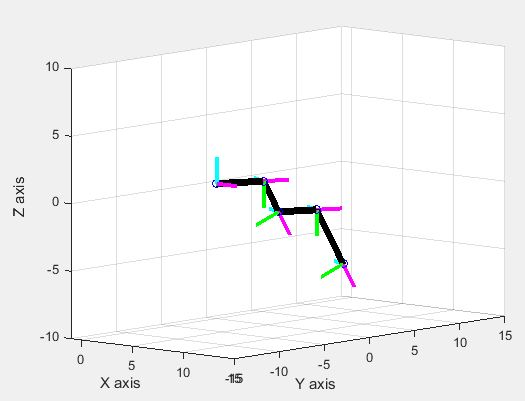
\includegraphics[width=0.5\textwidth]{matlabarm}
\caption{Arm graphed onto 3D image in Matlab.}
\label{fig:matlab}
\end{figure}

The inverse kinematics was tested using this model before testing on the real manipulator. The inverse kinematics equations along with the joint limits were programmed into a matlab function. The program could draw the resulting arm configuration for any desired end effector position in the workspace. For cases was not solvable the arm simply did not move, this was determined using the inverse kinematics feasibility test described in Chapter 3. The physical constraints were also programmed into the code to stop the arm for traveling outside of the physical angle limitations. Testing this code confirmed that the workspace of the manipulator is convex. This means that from one existing point in the workspace to other point in the workspace then the line between them is also in the workspace. This fact was use to create a trajectory from a starting position to a desired end position by calculating the linear path between them.

The next model was made to test the path planning code. In matlab obstacles were drawn on the 3D graph with the centers at the inputted obstacle value. The path planning algorithm then computed the path for the manipulator which was drawn through each configuration in the path. This model showed the algorithm to be able to consistently make it to the desired obstacle location with a smooth trajectory. The matlab simulation did not include any modeling of the gripper simply showing the path to the obstacle. An image of this simulation is shown in Figure \ref{fig:pathmatlab}.

\begin{figure}[h]
\centering
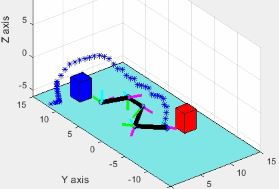
\includegraphics[width=0.5\textwidth]{pathmatlab}
\caption{Path planning simulation in matlab.}
\label{fig:pathmatlab}
\end{figure}

A more realistic model of the manipulator was created in the Virtual Robo Experimentation Platform (V-REP). This software includes physics engines which could more accurately simulated the manipulator at he goal objects reactions. First the servo and brackets 3D models were downloaded and the arm was assembled in Solidworks to create an accurate model of the manipulator. The 3D model was imported into V-REP and each servo set as a joint. Obstacles were created a similar size, shape, and weight as the real obstacles 3D printed for this project. The same matlab code was used to control the joint angles in V-REP. The simulation was then run and used to pick up objects. 

The V-REP simulation was not as reliable as the matlab simulation and a few code changes needed to be made to avoid the open gripper hitting the obstacles. There were also some problems with the objects flying out of the gripper. This seemed to  be a result of the physics engine and after a few adjustments to the object materials the simulation successfully picked up the object. An image of this simulation is shown in Figure \ref{fig:pathvrep}. The results of this simulation made it seem as though the path planning algorithm was likely to work with the real manipulator but would likely need some tuning to successfully grab objects. 

\begin{figure}
\centering
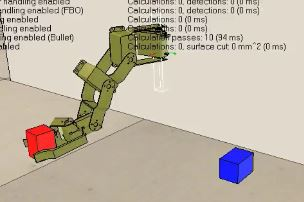
\includegraphics[width=0.5\textwidth]{pathplan}
\caption{Path planning model in V-REP.}
\label{fig:pathvrep}
\end{figure}
\chapter{Results}
Once all parts of this project were developed individually testing began on the physical manipulator. The main code for this project was written in python and used to call the image program to return the world coordinates of each known obstacle in the workspace. The program then calculated a path to the desired object while avoiding the others using the developed path planning code. The path was then sent over serial to the micro-controller which commanded the servos of the arm to the desired locations. 

The obstacles used to test the path planning were an orange cylinder, a blue square prism, and a green triangular prism. These objects can be seen in the figures of the image processing section.

Implementing this code made it easier to test many different object locations than it was with the modeled versions of the arm's path planning. There were a limited number of locations where obstacles could be placed that remained in the workspace of the manipulator. It was not possible to simply place an object anywhere near the manipulator and have it plan a path to it as some of the locations were not possible for it to reach.

For the obstacles within the reach of the arm's kinematics it could only pick up a few based on the two part path developed in the models. The arm would only successfully grab the obstacle when two conditions were met. The first was that the path's first approach was ended in an orientation pointing at the obstacle, rather than being at the side. The second condition was that the second part of the path, to actually do the grabbing did not cause the arm to hit the obstacle before grabbing. This problem is caused by the fact that the goal location cannot be both an obstacle and goal for the whole of path planning or the manipulator will never reach it. 

The first approach to fix this problem was to add a factor into the cost function for if the arm was pointing at the goal. The hope was that the arm would then calculated a path in which it was facing the goal and stop it from hitting the obstacle during the second part of the path planning. The issue with adding the orientation cost is that there is not enough flexibility in the manipulator workspace to get to a location and have the desired orientation. The result of adding this parameter is with a low tuning value that the arm ignores this orientation and simply takes longer to solve for the path it would have taken before, or with a higher tuning value cannot find a path within a reasonable amount of processing time. If the path calculations are not over after a minute there it does not seem to find a solution. There was no tuning value that could get the orientation parameter to improve the path planning.

The next approach was to set the end position of the first part of the path to a different location depending on the angle of the first joint. The goal is to place the arm at a position in which it is directly in front of the desired object. For example with an object directly to the front of the manipulator, at $\theta_1$ = around $0^o$ the best method was to send the manipulator to the coordinates $x_c -2 ,y_c , z_c$ where $x_c, y_c, z_c$ are the goal coordinates in inches. For $\theta_1$ values around $-90^o$ the formula was found to work best as $x_c, y_c -2, z_c$. For those in between a point two inches in from the x and y were used. For the negative angles the signs of the y were flipped. 

For the path planning algorithm to end it was required to find a distance where the arm was considered close enough to the point to stop the path planning. Since the angles were changed by a step size of three the arm would never perfectly reach the location. This was set to be within half an inch of the desired position. This means that there is some inaccuracy in the location of the end effector to the desired position. There is also some inaccuracy when calculated the position of the xyz coordinates. This accuracy is usually within a square inch of the actual location. Between these two there can be an error in the end effector location to a radius of one and a half square inches of the actual object center. Usually there is less error than this and the gripper is wide enough to grab the object for small amounts of error. 

The biggest issue of this system was the lack of feedback. The combination of error from the servos, camera location, and path planning results in a combined error of over an inch. This means that the manipulator often got close to the desired goal but not quite at the right position. The problem also arose of the error resulting in collisions with the arm and the objects. With feedback it would become much more possible to control this error resulting in a more reliable path planner. Having the gripper open as wide as possible while planning a path did help the reliability of actually grabbing the goal object, but also increased the chance of hitting other obstacles along the way.

Overall after some adjustments to the code this program was able to grab objects, while avoiding obstacles, for most locations in the workspace. With the limited workspace there is not always a path to find which can successfully grab the object without hitting it away. So while the path planner can find a smooth path to the object it was much harder to keep the arm in an orientation where it could actually pick up the object. The inaccuracy of the system was also a big contribution in the unreliable grasping.


\begin{figure}
    \centering
    \begin{subfigure}[b]{0.25\textwidth}
    	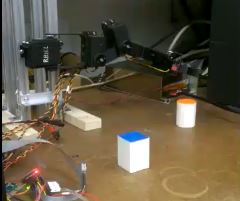
\includegraphics[width=\textwidth]{1}

   	 \end{subfigure}
   	 \quad
    \begin{subfigure}[b]{0.25\textwidth}
		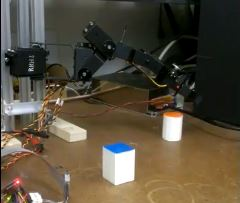
\includegraphics[width=\textwidth]{2}

    \end{subfigure}
    \quad %add desired spacing between images, e. g. ~, \quad, \qquad, \hfill etc.
    \begin{subfigure}[b]{0.25\textwidth}
        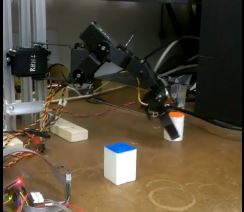
\includegraphics[width=\textwidth]{3}

    \end{subfigure}
    \quad
    \begin{subfigure}[b]{0.25\textwidth}
       	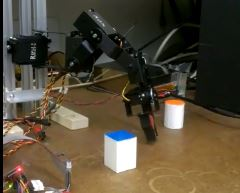
\includegraphics[width=\textwidth]{4}

   \end{subfigure}
    \quad
    \begin{subfigure}[b]{0.25\textwidth}
        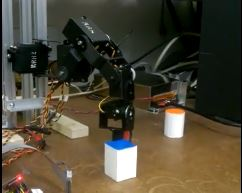
\includegraphics[width=\textwidth]{5}

    \end{subfigure}
    \quad
   	\begin{subfigure}[b]{0.25\textwidth}
        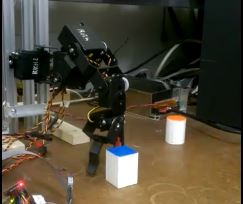
\includegraphics[width=\textwidth]{6}
    
   \end{subfigure}
   \quad
   \begin{subfigure}[b]{0.25\textwidth}
       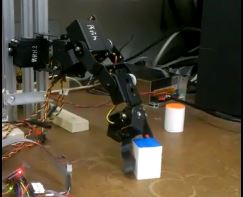
\includegraphics[width=\textwidth]{7}
        
   \end{subfigure}
   \quad
    \begin{subfigure}[b]{0.25\textwidth}
        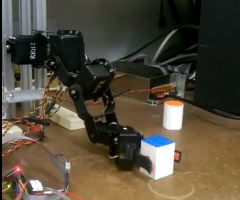
\includegraphics[width=\textwidth]{8}

    \end{subfigure}
    \quad
    \begin{subfigure}[b]{0.25\textwidth}
        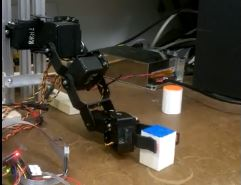
\includegraphics[width=\textwidth]{9}

    \end{subfigure}
    \quad
    \begin{subfigure}[b]{0.25\textwidth}
        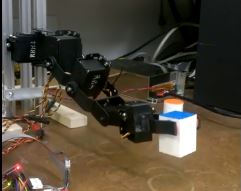
\includegraphics[width=\textwidth]{10}

    \end{subfigure}
    \quad
    \begin{subfigure}[b]{0.25\textwidth}
        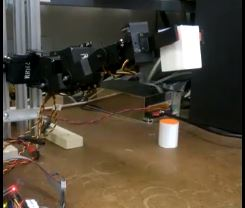
\includegraphics[width=\textwidth]{11}

    \end{subfigure}
    \quad
      %(or a blank line to force the subfigure onto a new line)
 	\caption{Manipulator moving through a planned path. }
 	\label{fig:images}
\end{figure}
\chapter{Conclusion}
Using robotic manipulators to pick up objects requires methods of path planning and workspace visualization. The more degrees of freedom a manipulator has the simpler the design of a path planning algorithm is but the more robust the result becomes. As seen by the results of this project this manipulator with for DOF has a fairly limited workspace, which becomes much more so if orientation is desired and not just an xyz position on space. While 4 DOF is plenty to move this manipulator to a location it is not enough to be able to grab objects well since more orientation is needed. 

If grabbing objects is desired for a manipulator with a small degrees of freedom, such as in this project, it becomes necessary to limit the locations where objects can be placed to be picked up. Rather than placing the object to any place in the workspace it must be put somewhere the correct orientation can be achieved. While this limits more robust applications this sort of design could be used in a manufacturing situation where objects can be placed at more exact locations that would work for the arm's configuration. For use in a more broad setting with less controlled object locations a manipulator with a higher degree of freedoms would become necessary.

Even with a more maneuverable configuration the lack of feedback in the system would still cause a reliability issue. With so much error coming from the servos and camera the path planner can find a path that works appropriately but does not work successfully. To develop a reliable path planner feedback is crucial.  

This project showed 3D cameras as an accurate way to visualize a workspace. Without some form of stereo camera or a lengthy calibration process it is difficult to obtain 3D data about a color image. The depth sensing camera is a powerful tool to overcome the difficulty of collecting 3D data. Since depth data can be directly mapped to a color image it is possible to get 3D world coordinates for all points within a color image. This method is also fairly accurate to within about half an inch in every direction making this method of gathering workspace data very practical. 

Computer vision and path planning can be used together to survey and move a manipulator through an environment. While the path planning and data gathering sections can be accurate the biggest challenge becomes physically grabbing the object. Getting to the location is nor the biggest issue, that becomes placing the manipulator in such a position accurately enough to have a gripper close around it without any part of the gripper hitting the object too far away. With more precise servos and more degrees of freedom this task could certainly be accomplished.


\bibliographystyle{IEEEtran}
\bibliography{IEEEabrv,bibliography}
\appendix

\chapter{CameraCode}\label{chap:sim_code}

\section{Object Tracking Method 1}
\lstinputlisting[basicstyle=\scriptsize,breaklines=true,language=C++]{./Code/camera1.cpp}
\section{Object Tracking Method 2}
\lstinputlisting[basicstyle=\scriptsize,breaklines=true,language=C++]{./Code/camera2.cpp}


\chapter{Path Planning and Communication}\label{chap:nao_code}

\section{Main Code}
\lstinputlisting[basicstyle=\scriptsize,breaklines=true,language=python]{./code/armTrackingMaster.py}
\section{Computer Communication}
\lstinputlisting[basicstyle=\scriptsize,breaklines=true,language=python]{./code/comms.py}
\section{Micro Controller Communication}
\lstinputlisting[basicstyle=\scriptsize,breaklines=true,language=python]{./code/communication.py}
\section{Path Planner}
\lstinputlisting[basicstyle=\scriptsize,breaklines=true,language=python]{./code/PathPlanner.py}
\section{Kinematics}
\lstinputlisting[basicstyle=\scriptsize,breaklines=true,language=python]{./code/arm.py}

\chapter{Arm Code}
\section{Main Code}
\lstinputlisting[basicstyle=\scriptsize,breaklines=true,language=C]{./code/arm_main.c}
\section{Arm Functions}
\lstinputlisting[basicstyle=\scriptsize,breaklines=true,language=C]{./code/arm.c}
\begin{thebibliography}{99}

\bibitem{darpa1}
	Open CV documentaion.
	Retrieved from \url{http://docs.opencv.org/}

\bibitem{darpa1}
	PCL documentaion.
	Retrieved from \url{http://pointclouds.org/documentation/}
	
\bibitem{darpa1}
	DepthsenseSDK documentaion.
	Retrieved from \url{http://www.softkinetic.com/Support}
	
\bibitem{zmp_human1}
	Kristoffer Aasland,
	(2008).
	\emph{Optimal 3D Path Planning for a 9 DOF
	Robot Manipulator with Collision
	Avoidance}
	Retrieved from
	\url{http://www.diva-portal.org/smash/get/diva2:347626/FULLTEXT01.pdf}
	
\bibitem{zmp_human1}
	Mohamed Abdellatif,
	(2008).
	\emph{Effect of Color Pre-Processing on Color-Based Object Detection}
	Retrieved from
	\url{http://www.researchgate.net/profile/Mohamed_Abdellatif3/publication/248390823_Effect_of_Color_Pre-Processing_on_Color-Based_Object_Detection/links/02e7e51de87e9efc3f000000.pdf}
	
\bibitem{zmp_human1}
	Khaled Alhamzi, Mohammed Elmogy, Sherif Barakat,
	(2014).
	\emph{3D Object Recognition Based on Image Features: A Survey}
	Retrieved from
	\url{http://www.academia.edu/7188944/3D_Object_Recognition_Based_on_Image_Features_A_Survey}
	
\bibitem{zmp_human1}
	G. J. García, P. Gil, D. Llácer, F. Torres,
	(2012).
	\emph{Guidance of Robot Arms using Depth Data from RGB-D Camera}
	Retrieved from
	\url{http://rua.ua.es/dspace/bitstream/10045/30156/1/ICINCO_2013_154_CR.pdf}	
\end{thebibliography}
%\include{bib}
\end{document}